\documentclass[12pt, a4paper, dutch]{article}

\usepackage[margin=1in]{geometry}
\usepackage{circuitikz}
\usepackage{float}
\usepackage{babel}
\usepackage{siunitx}
\usepackage{amsmath}
\usepackage{scalerel}
\usepackage{csquotes}
\usepackage{parskip}
\usepackage{unicode-math}
\usepackage{fontspec}
\usepackage{tabularx}
\usepackage{booktabs}
\usepackage{graphicx}
\usepackage{pgfplots}
\usepackage{color}
\usepackage{hyperref}

\setmainfont{TeX Gyre Schola}
\setmathfont{TeX Gyre Schola Math}
\setmonofont{JetBrainsMono Nerd Font}
\sisetup{
	group-separator = {.},
	output-decimal-marker = {,}
}

\pgfplotsset{compat=newest}

\usetikzlibrary{calc}
\usetikzlibrary{shapes.geometric}
\usetikzlibrary{arrows.meta,arrows}
\usetikzlibrary{positioning}
\tikzset{
	initial/.style={circle, fill},
	final/.style={solid, double=white, circle, fill, thick, draw},
	decision/.style={diamond, black, draw},
	action/.style={rectangle, draw, rounded corners, align=center},
	arrow/.style={draw, -{Latex[length=3mm]}, thick, rounded corners}
}

\bigskipamount=7mm
\medskipamount=4mm
\parindent=0mm

\begin{document}

\begin{center}
\textbf{Ontwerp} \hspace{2mm} project ledcube \hfill \textbf{Loek Le Blansch}
(2180996)\\
\today \hfill \textbf{Sybren van den Heuvel} (21.....)
\end{center}

\medskip

Dit document maakt gebruik van hyperlinks, dus je kunt klikken op de blokken met
\emph{benadrukte tekst} om naar de definitie van dat blok te gaan.

\section{Software ontwerp}

\subsection*{Overzicht}\label{overzicht}
\begin{center}
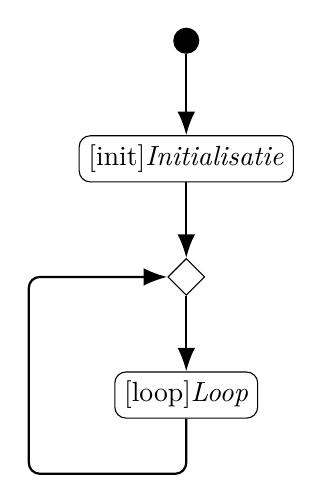
\begin{tikzpicture}[node distance=1.5cm]
\node[initial] (initial) at (0,0) {};
\node[action, below of = initial] (setup) {\hyperref[init]{\emph{Initialisatie}}};
\node[decision, below of = setup] (comb) {};
\node[action, below of = comb] (loop) {\hyperref[loop]{\emph{Loop}}};

\draw [arrow] (initial) -- (setup);
\draw [arrow] (setup) -- (comb);
\draw [arrow] (comb) -- (loop);
\draw [arrow] (loop) -- ++(0, -1) -- ++(-2, 0) |- (comb);

\end{tikzpicture}
\end{center}


\subsection*{Initialisatie}\label{init}
\begin{center}
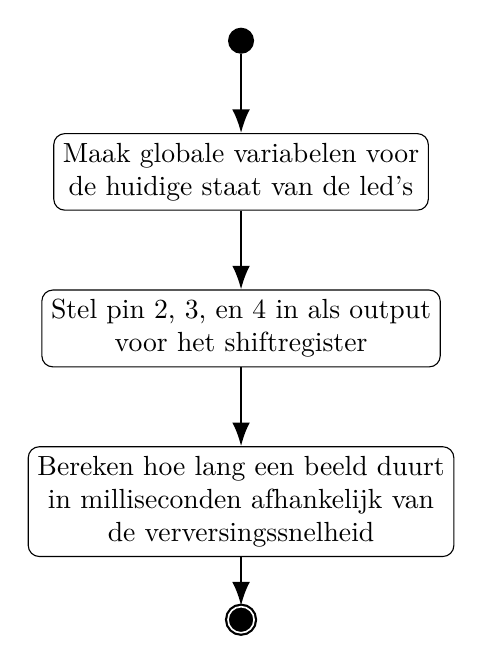
\begin{tikzpicture}[node distance=1.5cm]
\node[initial] (initial) at (0,0) {};

\node[action, below = 1cm of initial] (mkvars) {Maak globale variabelen voor\\de
	huidige staat van de led's};

\node[action, below = 1cm of mkvars] (pinmode) {Stel pin 2, 3, en 4 in als
	output\\voor het shiftregister};

\node[action, below = 1cm of pinmode] (frametimecalc) {Bereken hoe lang een beeld
	duurt\\in milliseconden afhankelijk van\\de verversingssnelheid};

\node[final, below of = frametimecalc] (final) {};

\draw [arrow] (initial) -- (mkvars);
\draw [arrow] (mkvars) -- (pinmode);
\draw [arrow] (pinmode) -- (frametimecalc);
\draw [arrow] (frametimecalc) -- (final);

\end{tikzpicture}
\end{center}


\subsection*{Loop}\label{loop}
\begin{center}
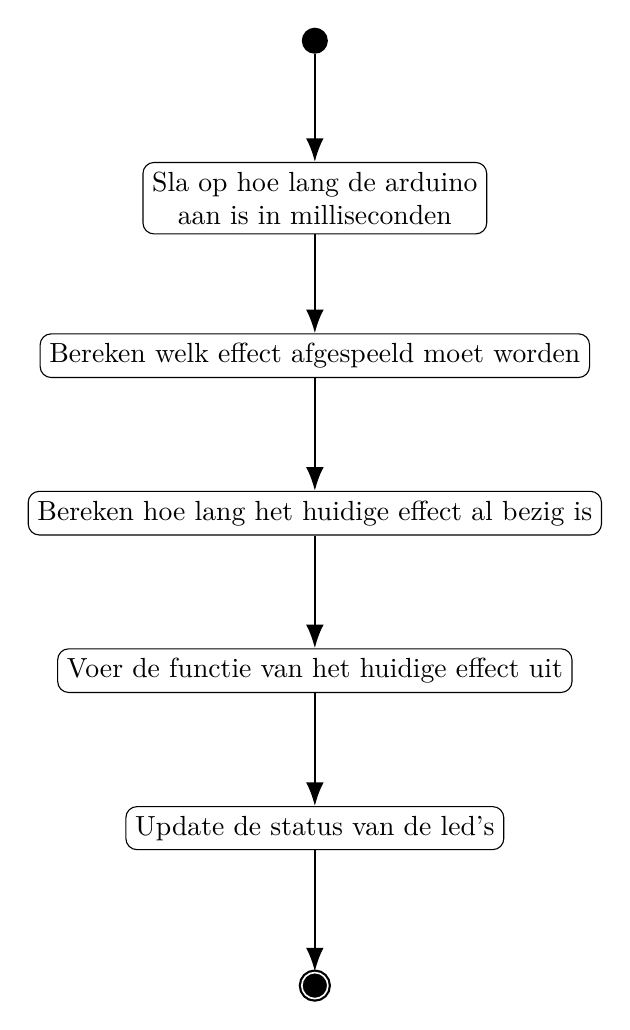
\begin{tikzpicture}[node distance=2cm]
\node[initial] (initial) at (0,0) {};

\node[action, below of = initial] (gettime)
	{Sla op hoe lang de arduino\\aan is in milliseconden};

\node[action, below of = gettime] (calcfxindex)
	{Bereken welk effect afgespeeld moet worden};

\node[action, below of = calcfxindex] (calcfxtime)
	{Bereken hoe lang het huidige effect al bezig is};

\node[action, below of = calcfxtime] (fxexec)
	{Voer de functie van het huidige effect uit};

\node[action, below of = fxexec] (updateregs)
	{Update de status van de led's};

\node[final, below of = updateregs] (final) {};

\draw [arrow] (initial) -- (gettime);
\draw [arrow] (gettime) -- (calcfxindex);
\draw [arrow] (calcfxindex) -- (calcfxtime);
\draw [arrow] (calcfxtime) -- (fxexec);
\draw [arrow] (fxexec) -- (updateregs);
\draw [arrow] (updateregs) -- (final);

\end{tikzpicture}
\end{center}

\section{Hardware}

\subsection{Schema}

\begin{center}
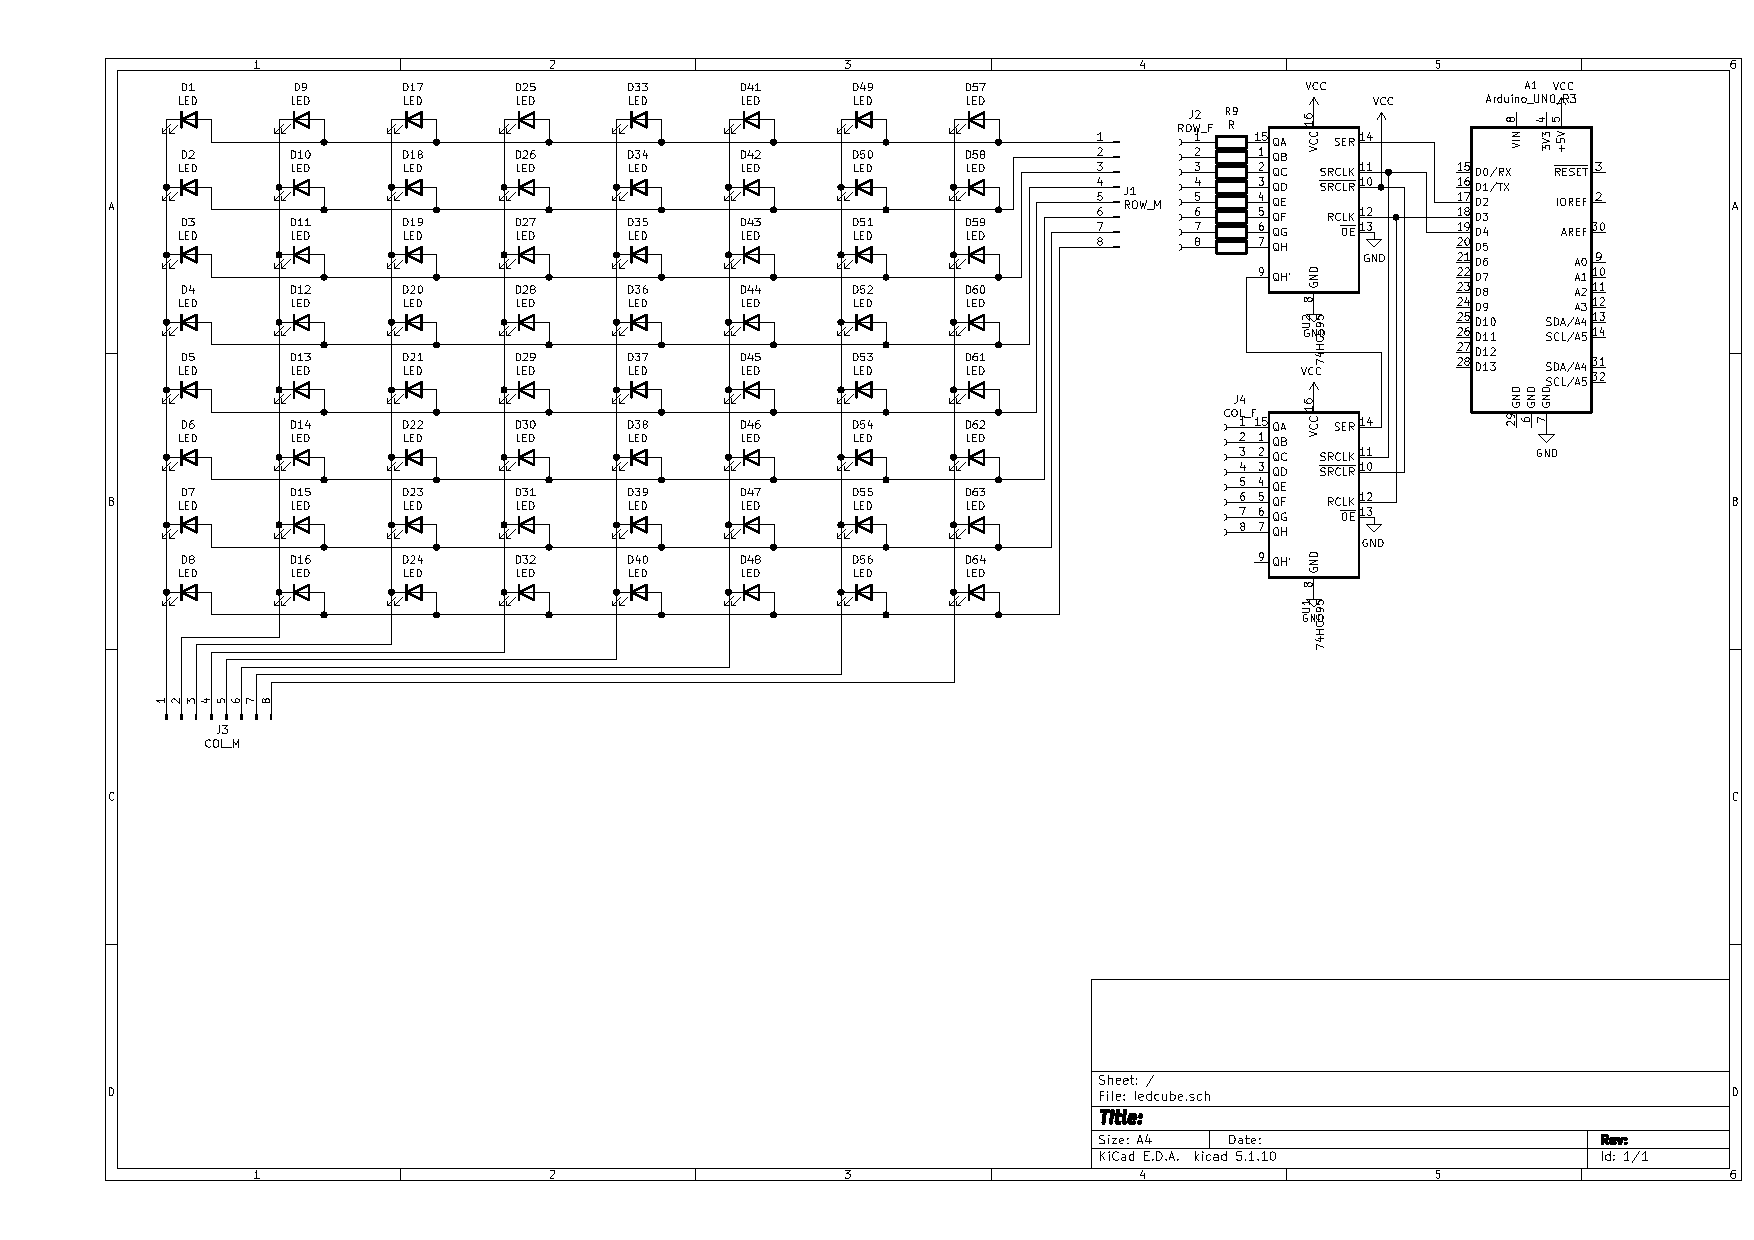
\includegraphics[
	clip,
	trim=21mm 83mm 22mm 13mm,
	width=\textwidth
]{./schema.pdf}
\end{center}

\subsection{PCB}
\begin{center}
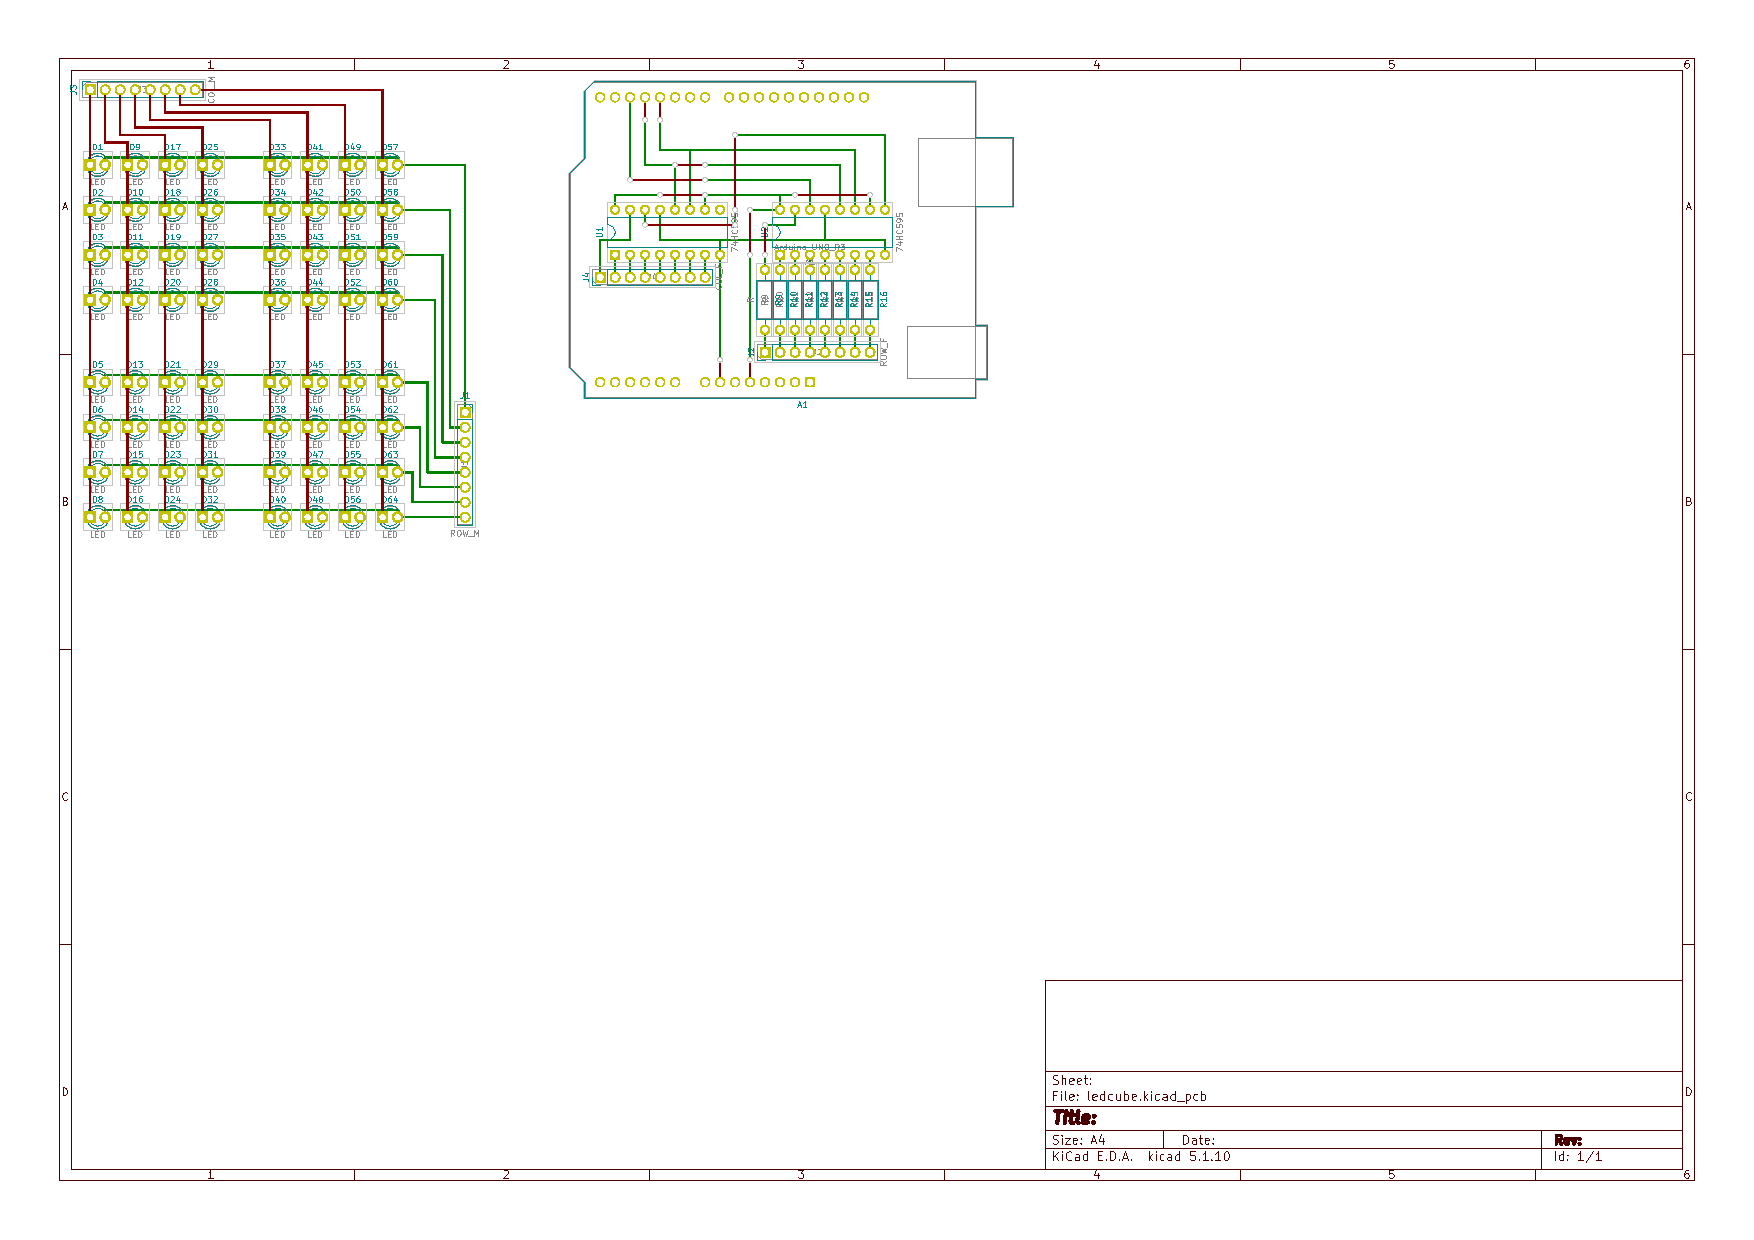
\includegraphics[
	clip,
	trim=13mm 119mm 124mm 13mm,
	width=\textwidth
]{./pcb.pdf}
\end{center}

\subsection{Bedrading (3D)}

Dit is een 3D-weergave van de bedrading van de led cube. In deze weergave zie je
duidelijk dat de led cube bestaat uit een 8$\times$8-matrix die twee keer is
dubbelgevouwd. Hier zijn de roze verbindingen de anode's van de led's, en de blauwe
de cathode's.

\begin{center}
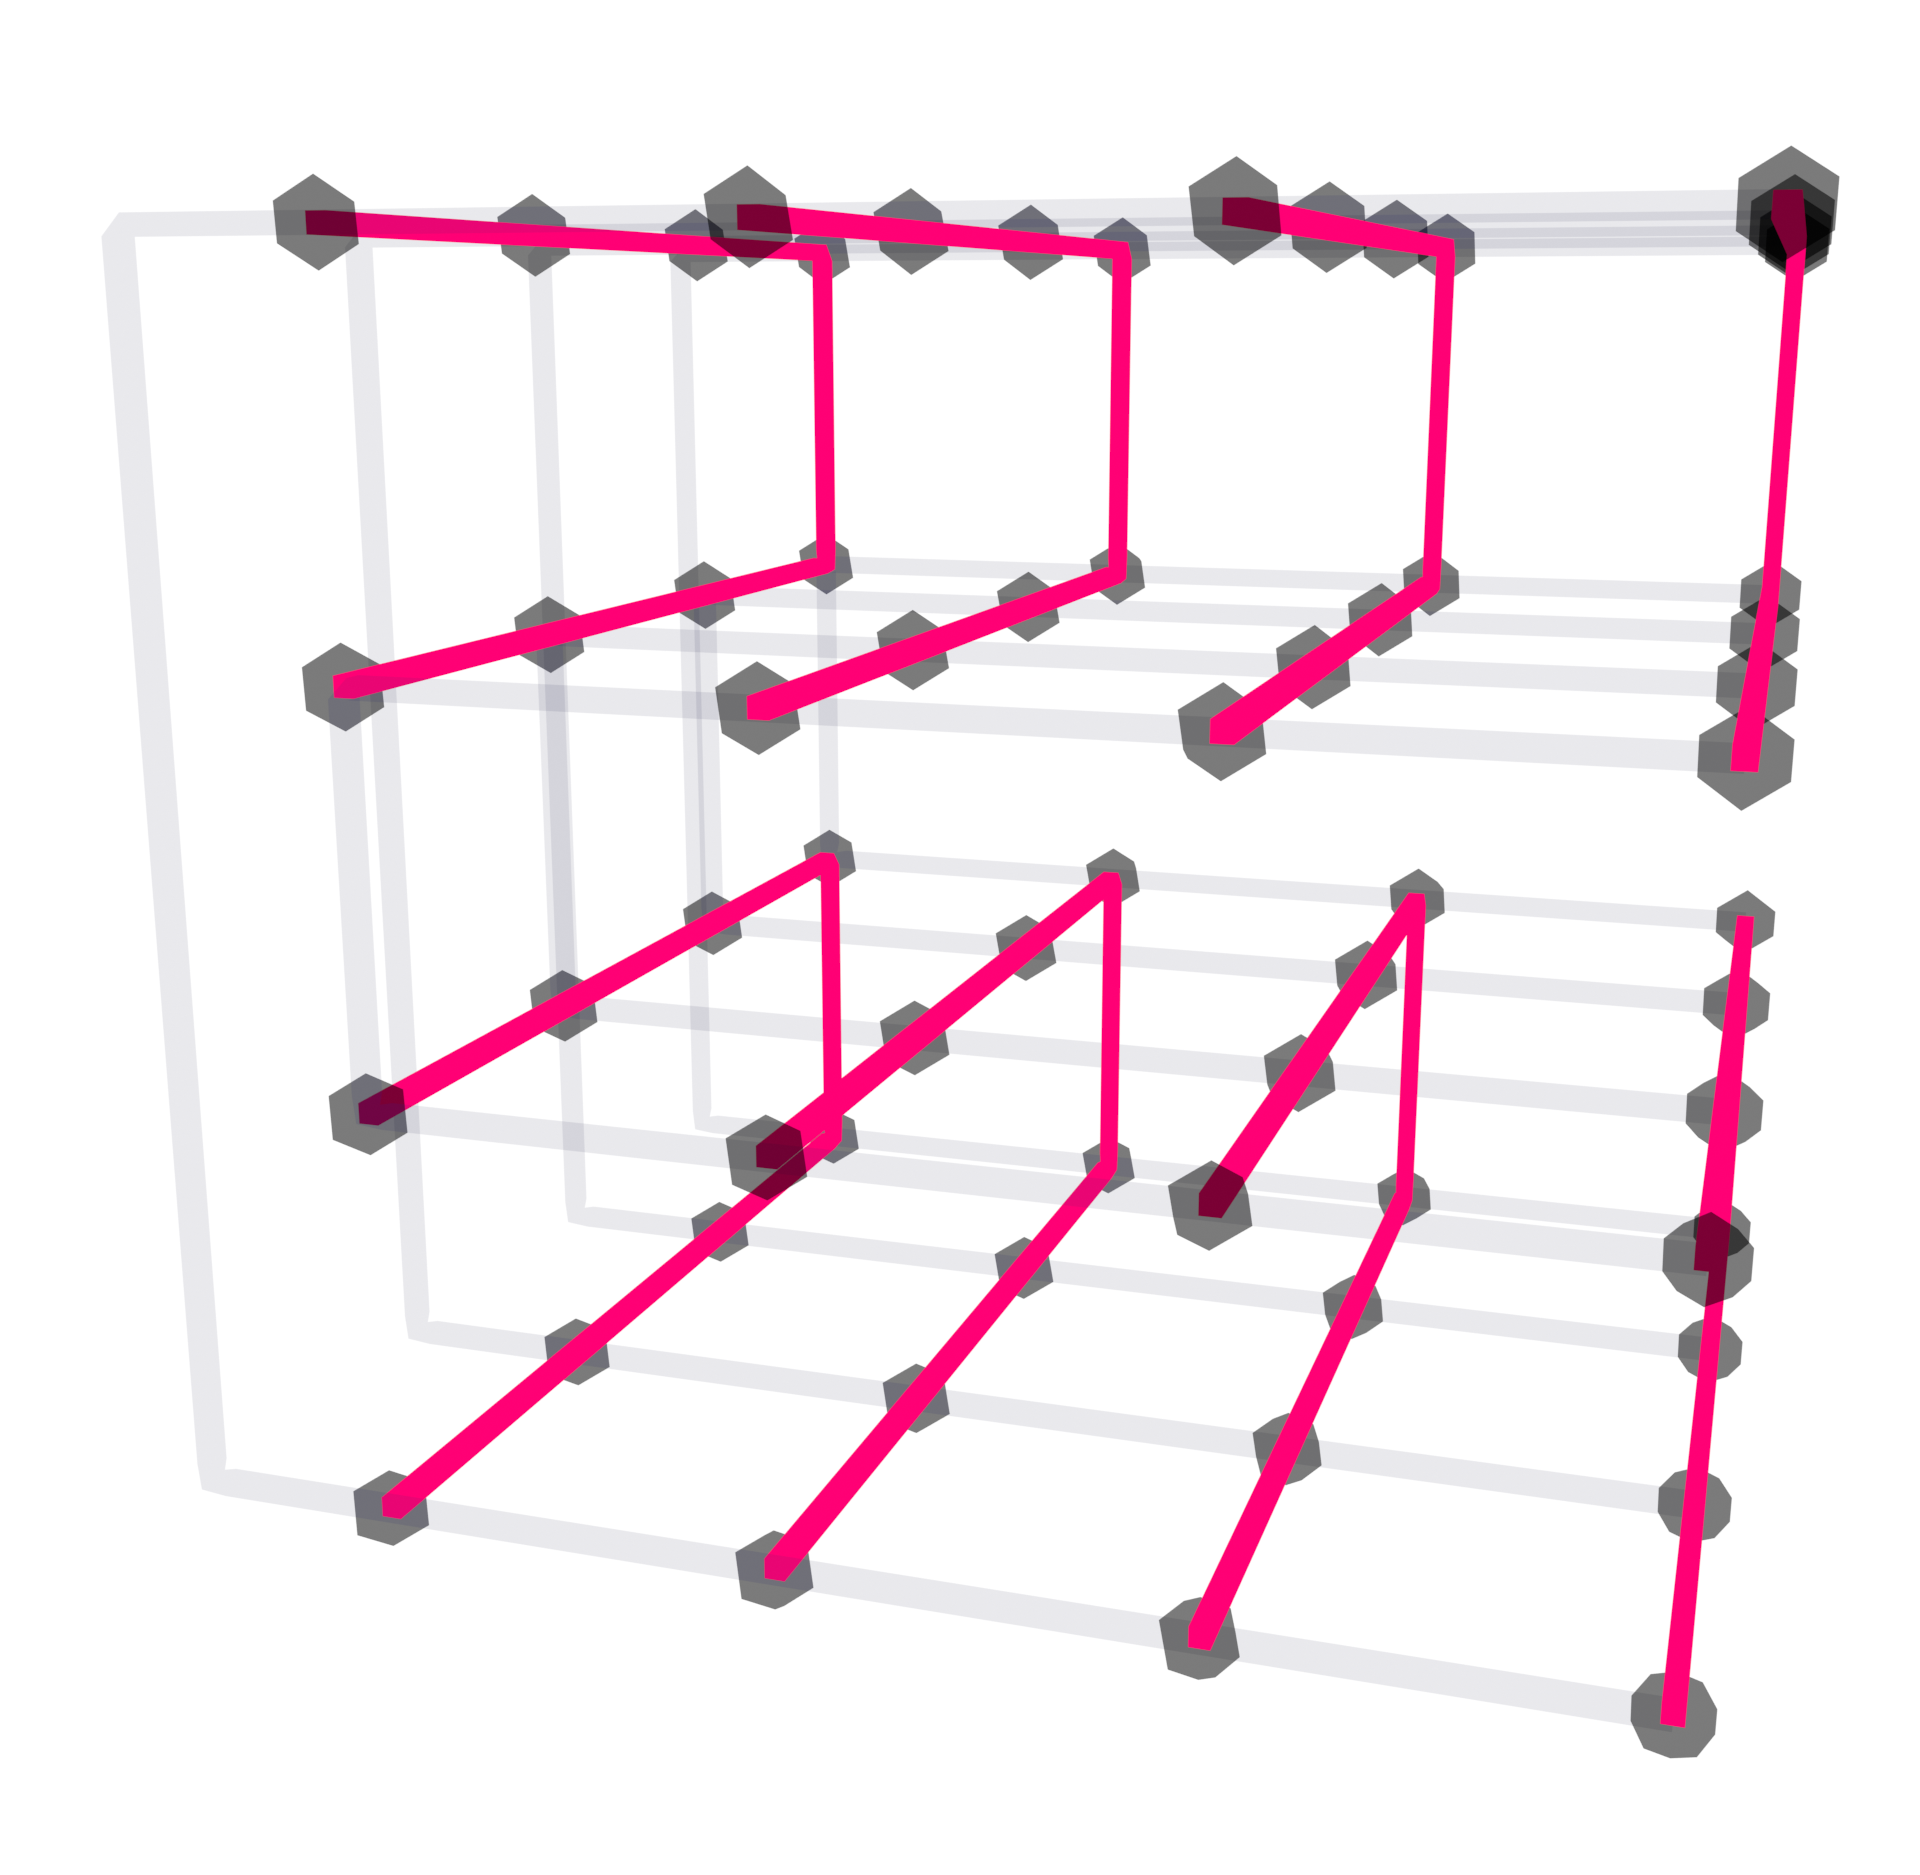
\includegraphics[
	width=0.4\textwidth
]{./red.png}
\hspace{1cm}
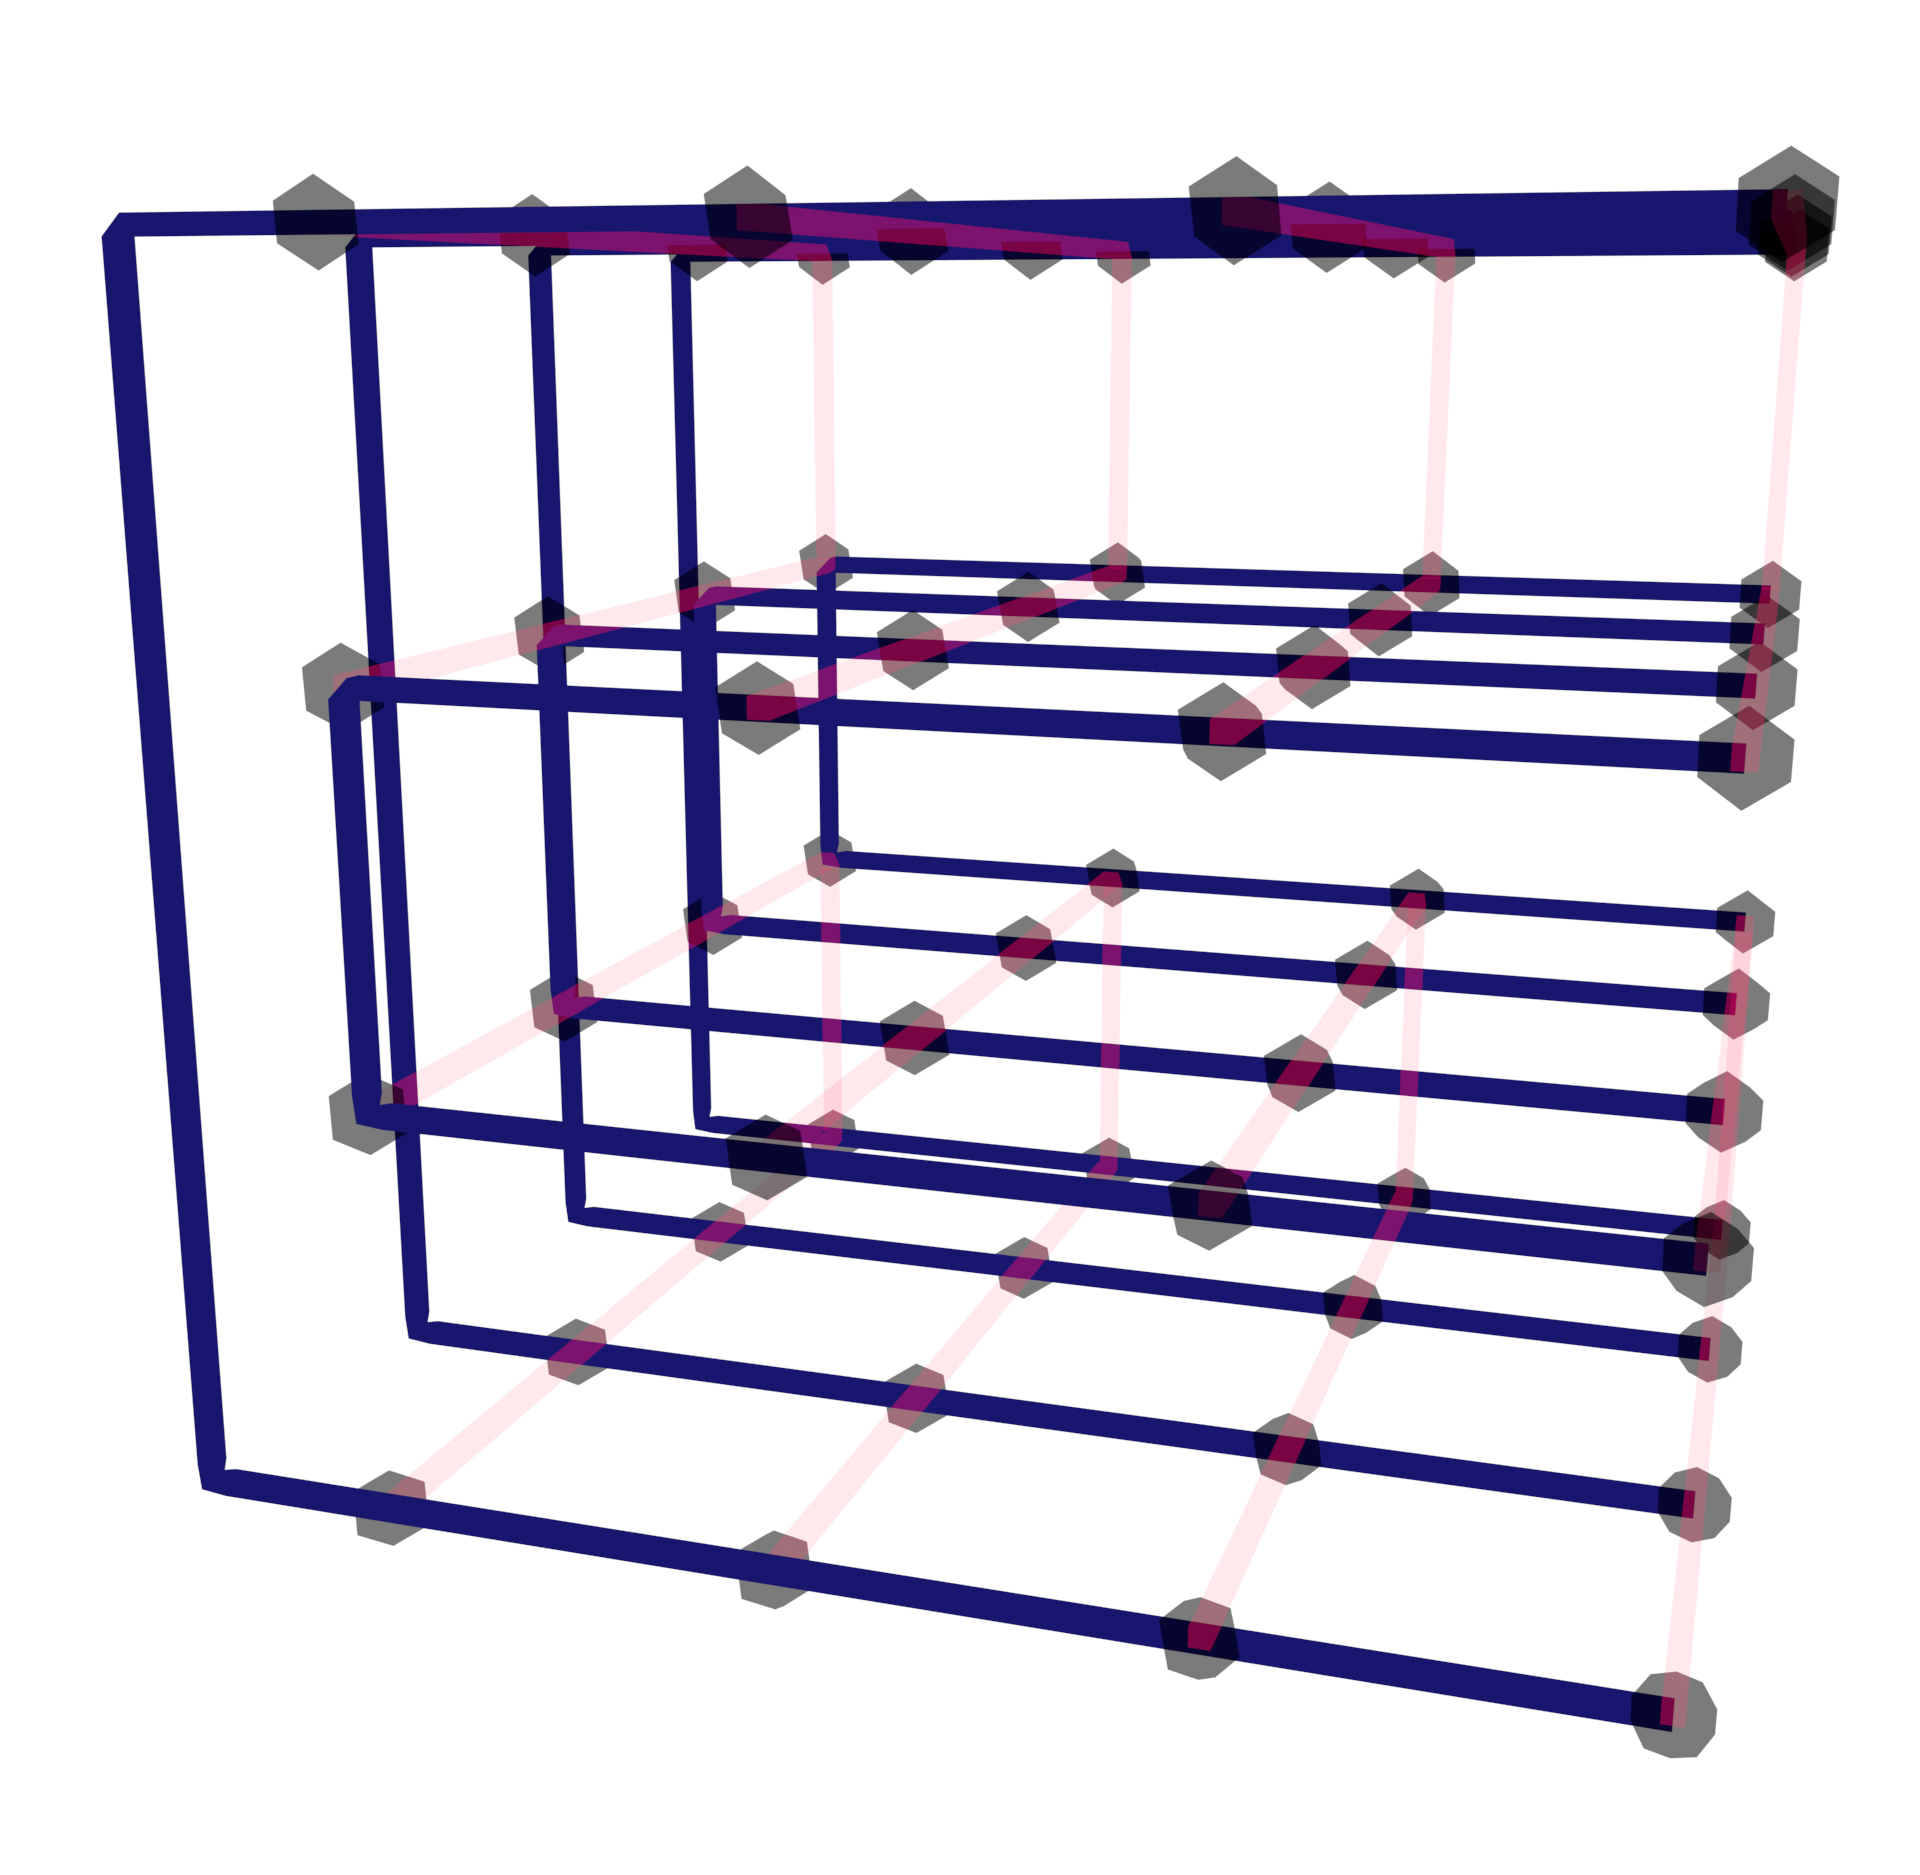
\includegraphics[
	width=0.4\textwidth
]{./blue.png}
\end{center}

\end{document}
